%
% File acl2012.tex
%
% Contact: Maggie Li (cswjli@comp.polyu.edu.hk), Michael White (mwhite@ling.osu.edu)
%%
%% Based on the style files for ACL2008 by Joakim Nivre and Noah Smith
%% and that of ACL2010 by Jing-Shin Chang and Philipp Koehn


\documentclass[11pt]{article}
\usepackage{acl2012}
\usepackage{times}
\usepackage{latexsym}
\usepackage{amsmath}
\usepackage{graphicx}
\usepackage{multirow}
\usepackage{enumerate}
\usepackage{url}
\DeclareMathOperator*{\argmax}{arg\,max}
\setlength\titlebox{3.5cm}    % Expanding the titlebox
\newcommand{\ignore}[1]{}

%\newcommand{\B}{\mathcal{B}} 

\title{A Model of Random Walks on Bipartite Graph for Classification Problems}

\ignore{
\author{First Author \\
}
}

\date{}

\begin{document}
\maketitle
\begin{abstract}
We introduce a general framework of semi-supervised graphical model that is
applicable to any classification tasks that can be represented with norminal
features, requiring only a handhul of labeled examples.
We conducted experiments on three different NLP tasks: prepositional phrase 
attachment, named entity classification, and domain-specific terminology extraction. 
We show both theoretically and empirically how the graph structure helps making 
use of large amount of unlabeled data.
Based on the empirically study of underlying correlations between graph structures and
classification performance, we incorporate active learning techniques to 
achieve the best learning rate with minimum requirement on labeled data. 
\end{abstract}

%%%%%%%%%%%%%%%%%%%%%
\section{Introduction}

Semi-supervised learning on graphs is a direction that has drawn great
attentions from NLP researchers. %The general idea behind various semi-supervised
%graphical methods is constructing a graph can be automated, while 
An abstract framework that we have often seen in graph based NLP is constructing
a graph in which each vertex represents an instance which can
be a word, a concept, a sentence, an article etc. Edges
are connected and weighted according to some manually selected
function that defines the closeness or similarity of any two instances in the
context of the application. 
One possible usage of the graph is to predict the
property (label) of a node via comparing the distances of this node to other
nodes with known labels. For example, //add a citation here

Another information we can obtain from the graph is the importance of a node.
We see algorithms such as PageRank\cite{}, HITS\cite{}, and graph based
summarization systems\cite{} .




In this paper, we introduce a model that shares with many other graphical
methods the idea of encoding similarities between instances into a graphical
structure and learning from unlabeled instances, while presents its novelty in
the following two aspects. First, the graph is bipartite. Example nodes and
feature nodes form two subsets of the bipartite graph. We will show later this
can be equivalently converted to a graph consisting of only example nodes
assuming a special edge weight definition. This
assumption simplifies the graph construction by a factor of the number of example nodes. 
Second, we observe from experiment that when the labeled training size is very
small compared to the entire graph, performance of the model is unstable due to the
randomness in sampling training examples. We extend the model with an active
learning technique that intellegently chooses the most ``informative'' unlabeled
examples to learn. Such property is well appreciated in applications where
labeled examples are very expensive to obtain.  


%%%%%%%%%%%%%%%%%%%%%

\begin{figure*}[ht!]
\centering
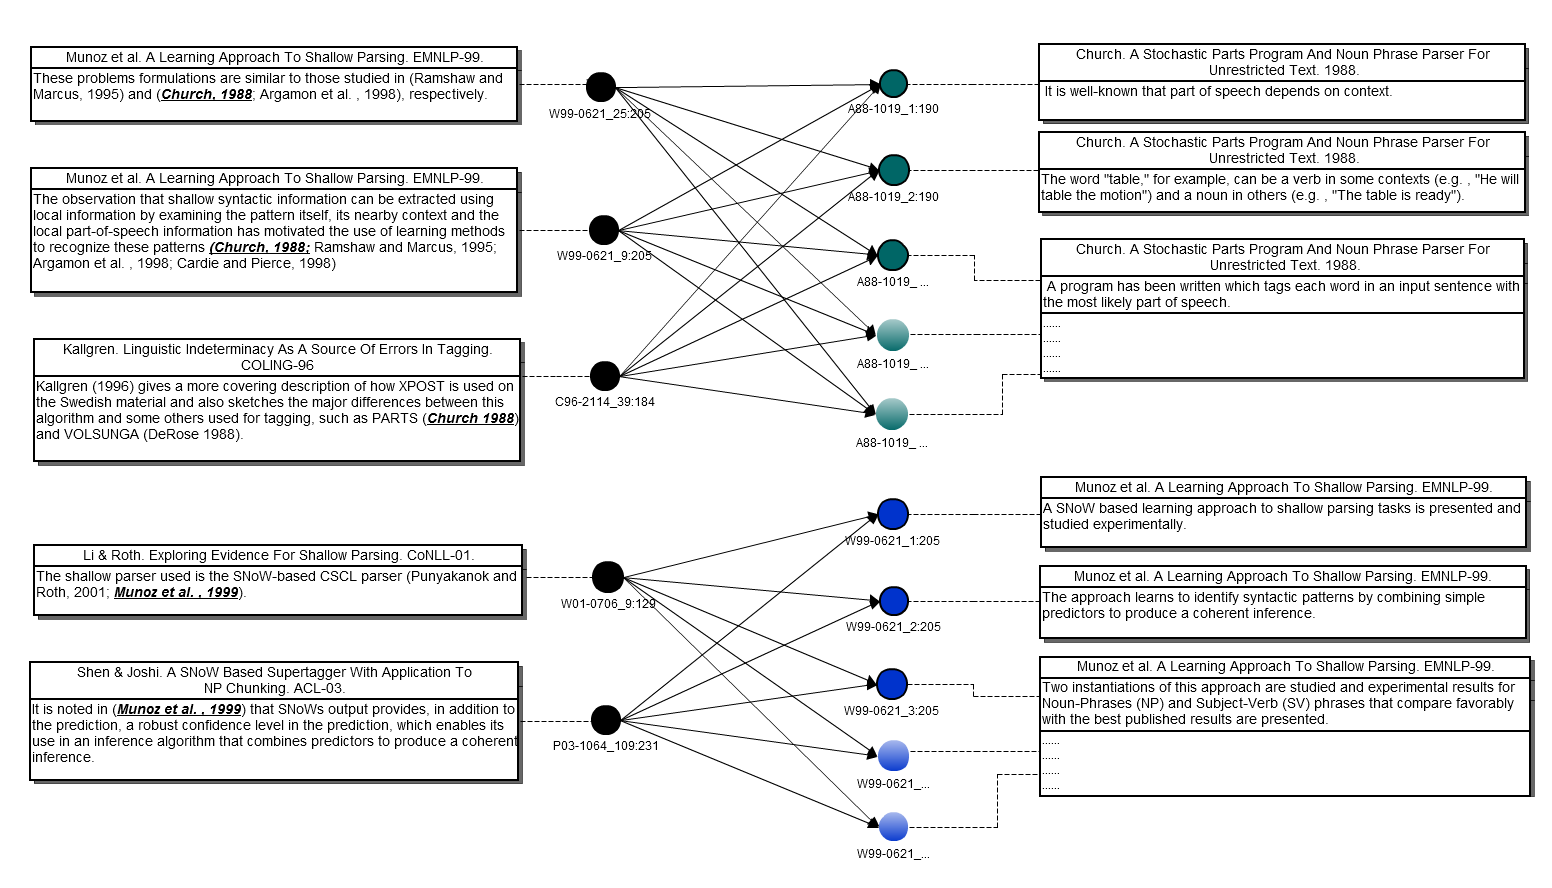
\includegraphics[width=\textwidth]{graph/bipartite_graph.png}
\caption{A mini-model of the bi-partite graph for Chapter 5 (Part-of-Speech Tagging)}\label{fig:bi}
\end{figure*}

\begin{table*}
\centering
{\scriptsize
\begin{tabular}{|l|cc|rrr|}
  \hline
 Chapter & src & cit & $|\B_L|$ & $|\B_R|$ & $E_\B$ \\
  \hline \hline
 Words and Transducers & 14&     255&    489&    $3,484$ &   $202,940$ \\
 N-grams & 5&      73&     97&     $2,083$ &   $32,690$ \\
 Part-of-Speech Tagging & 16&     657&    $1,261$ &   $3,385$ &   $344,886$\\
 Hidden Markov and Maximum Entropy Models & 2&      432&    659&    525&    $187,905$\\
 Phonetics & 1&      12&     81&     216&    $17,496$\\
 Speech Synthesis & 4&      54&     126&    920&    $29,357$\\
 Automatic Speech Recognition & 2&      27&     103&    401&    $21,566$\\
 Speech Recognition: Advanced Topics & 7&      189&    445&    $2,007$&   $96,467$\\
 Syntactic Parsing & 4&      131&    246&    763&    $63,673$\\
 Dialog and Conversational Agents & 11&     170&    368&    $3,745$ &   $114,281$\\
  \hline
\end{tabular}}
\caption{List of chapter historical notes used in our experiments together with the number of source papers extracted from historical notes (src), the number of citing papers extracted from AAN (cit), size of the left ($\B_L$) and right ($\B_R$) components in the bi-partite graph, and number of edges in the graph ($E_\B$).}\label{tbl:chapters}
\end{table*}

\section{Approach}
\label{sec:approach}

Previous work on scientific survey generation have compared surveys that are generated from different sources such as citations and source paper texts~\cite{Qazvinian&Radev08a,mei&zhai08,mohammad-EtAl:2009:NAACLHLT09}. However, none of these approaches combine these heterogeneous information sources to produce automatic surveys. 

In our approach, we investigate the usefulness of combining different information sources and producing summaries that are both affected by source paper text and citation information. For a set of papers in the same scientific topic, we extract survey worthy sentences from the source texts that cover contributions recognized by other scholars in citations, and extract citations that cover contributions that are recognized by the authors in the source text.

In our algorithm, we model the set of papers in a scientific topic $t$ as a bi-partite graph, $\B$ with a left and a right component ($\B_L$, $\B_R$). Each node in $\B_L$ is a citation sentence to one or more papers in $t$ extracted from AAN, and each node in $\B_R$, represents a sentence extracted from the source text of a paper in $t$. We construct the edges in $\B$ by connecting each citing sentence to all the source sentences in the papers it cites. Each edge in $\B$ is assigned a weight equal to the cosine similarity of the TF-IDF term vectors of the two sentences it connects. 
Figure~\ref{fig:bi} illustrates part of the bi-partite graph for built for the ``Part-of-Speech Tagging'' chapter in the JM book.

To build the summaries we are interested in citations and source sentences that cover important contributions in the given scientific topics. Intuitively, contributions that both the paper authors and other scholars recognize as significant are important and should be extracted. Surveyor extracts citations that cover important contributions mentioned in the source papers as well as source sentences that discuss important factoids recognized by others in citations.


\subsection{Ranking}
The inherent duality in the source papers and citations suggests that the problem could be addressed by applying the HITS algorithm~\cite{Kleinberg:1999} to iteratively assign hub and authority scores to citations and source sentences respectively. The induction process is as follows. Each citation sentence $c\in \B_L$ is associated with a hub score $h_c$, and each source sentence $s\in \B_R$ is associated with an authority score $a_s$. These scores are initialized with a value of $1.0$.  Hub and authority scores are iteratively updated using the following equations.

{\small
\begin{eqnarray}
\label{hits1} a^{(i+1)}_s = \sum_{c\in nei(s)} \frac{h^{(i)}_c}{H^{(i)}}
\end{eqnarray}
}
{\small
\begin{eqnarray}
\label{hits2} h^{(i+1)}_c = \sum_{s\in nei(c)} \frac{a^{(i)}_s}{A^{(i)}}
\end{eqnarray}
}

where a source sentence $s$ is in a citation sentence, $c$'s neighborhood ($s\in nei(c)$) if there is an edge between $s$ and $c$ in $\B$ ($c$ cites the paper that contains $s$), and their cosine similarity is greater than a threshold (i.e., $cos(s,c) > \theta$). Here, $H^{(i)}$ and $A^{(i)}$ are normalization factors:

{\small
\begin{eqnarray}
H^{(i)} = (\sum_{c\in \B_L} {h^{(i)}_c}^2)^{1/2}\\
A^{(i)} = (\sum_{s\in \B_R} {a^{(i)}_s}^2)^{1/2}
\end{eqnarray}}

In our experiments, we set $\theta = 0.1$. This ranking gives us top authorities (source sentences) and top hubs (citations) with which we build two different summaries: {\bf $\textrm{HITS}_\textrm{src}$} and {\bf $\textrm{HITS}_\textrm{cit}$}. Although these summaries are built from different sources (i.e., source papers and citations) they are affected by each other. In other words, the scores and thus extraction of top citations affects the extraction of top source sentences and vice versa. 


\subsection{Adding Weights}
In previous section, we described the basic version of our system in which the edges are considered as binary connections (if the cosine similarity is above a threshold). We would like to investigate the effect of similarity on sentence extraction. In other words, instead of applying a threshold we use the actual edge weights and modify Equations \ref{hits1}, \ref{hits2} as follows.

{\small
\begin{eqnarray}
\label{whits1} a^{(i+1)}_s = \sum_{c\in nei(s)} \frac{w_{cs} \cdot  h^{(i)}_c}{H^{(i)}}\\
\label{whits2} h^{(i+1)}_c = \sum_{s\in nei(c)} \frac{w_{sc} \cdot a^{(i)}_s}{A^{(i)}}
\end{eqnarray}}

where $w_{sc}$ is the is the edge weight between vertices $s$ and $c$, calculated as the TF-IDF based cosine similarity between their corresponding sentences.

Intuitively, this modification will take into account the similarity of sentence with its neighbors rather than the number of connections, and would result in summaries that contain more \emph{lexically} salient sentences. 
The weighted ranking gives us top authorities (source sentences) and top hubs (citations) with which we build two different summaries: {\bf $\textrm{HITS}_\textrm{src} \textrm{ with weights}$} and {\bf $\textrm{HITS}_\textrm{cit} \textrm{with weights}$}.

\subsection{Citation Bias}
The downside of the current HITS-based sentence extraction is that it assumes equal importance for the papers in a given topic. However, contributions from highly cited papers are intuitively more important. To address this issue, we propose an improvement inspired by~\cite{Mei&al2010} and modify equations \ref{hits1}, \ref{hits2} to include a prior distribution of prestige.

{\small
\begin{eqnarray}
\label{phits1} a^{(i+1)}_s = (1- \lambda) \cdot p^\ast(s) + \lambda \cdot \sum_{c\in nei(s)} \frac{h^{(i)}_c}{H^{(i)}}\\
\label{phits2} h^{(i+1)}_c = (1- \lambda) \cdot p^\ast(c) + \lambda \cdot \sum_{s\in nei(c)} \frac{a^{(i)}_s}{A^{(i)}}
\end{eqnarray}}

Here, $p^\ast(v)$ is a distribution which represents the prior preference of vertex $v$. When $p^\ast(v)$ is uniform, the left component is similar to the random jumping probabilities in PageRank. Other possible choices for $p^\ast(v)$ include a topic sensitive distribution, inspired by personalized jumping in personalized PageRank~\cite{Haveliwala2002,haveliwala2003topic}. 
In Equations~\ref{phits1},~\ref{phits2} $\lambda$ obtains a value between $0$ and $1$. When $\lambda = 1$, Equations~\ref{phits1},~\ref{phits2} lead to the standard HITS algorithm. In our experiments, we set $\lambda = 0.75$. 

The prior distribution allows us to favor citation sentences that are from more impactful papers. Therefore we define the prior distributions as the normalized citation frequency of the paper 

{\small
\begin{eqnarray}
p^\ast (v) = \frac{C_v + 1}{\sum_{v\in \B} C_v + |\B|} 
\end{eqnarray}}

where $C_v$ is the number of citations to the paper that contains sentence $v$.  
Equations~\ref{phits1},~\ref{phits2} give us top authorities (source sentences) and top hubs (citations) with which we build two different summaries:  {\bf $\textrm{HITS}_\textrm{src} \textrm{ with priors}$} and {\bf $\textrm{HITS}_\textrm{cit} \textrm{with priors}$}. 


%%%%%%%%%%%%%%%%%%%%%
\section{Active Learning}


Observations in a pilot experiment on the
preporsitional phrase attachment dataset motivated applying 
active learning.
In this section, we first briefly describe the PP
attachment classification task, dataset, and results form the pilot experiment.
Then we present the active learning algorithm.

\subsection{PP Attachment Dataset}\label{ppdata}

1) ppattach disambiguation

2) dataset

3) state-of-art, backoff method

\subsection{Pilot Experiment}

use basic tumbl model

plot: learning curve from 10 to 1000 training size 

plot: uncertianty - when sample size is small (e.g. 10 , 50) performance

variance is large, motivate a method to better choose examples to be labeled


\subsection{Algorithm with Active Learning}

// need to fill in after experiments



\section{Experiments} \lable{sec:experiment}

\subsection{PP attachemnt dataset}


1) baseline: backoff method

2) tumbl, randomly pick labeled examples

3) active learning

Todo: describe baseline, describe experiment settings

plot accuracy of 3 methods with different training size
%We use the backoff method \cite{} as our baseline, which is one of the that
%doesn't require.


\subsection{Named Entity Classification}

1) describe task and dataset

2) describe baseline DLCoTrain

3) experiment with NEC data

4) experiment DLCoTrain and tumbl on ppattach set

5) analysis


\subsection{AAN Terminology Extraction}

Not sure about this, if time is limited, show only preliminary
results, no comparison w/ other methods.

%%%%%%%%%%%%%%%%%%%%%
\section{Related Work}

1) Relation to Zhu's method harmonic function and Gaussian fields

-- distribution assumption

Zhu's method assumes Gaussian fields, the propability distribution of random
walk is a continuous Gaussian distribution on the reverse of the distance
between any two nodes. The graph is fully connected. 
It is a good model when the geometric distance is well defined.

In the bipartite graph model, the propability of one random step is propotional to the number of
common features shared by the two example nodes. It is actually the dot product
of two examples (recall that an example is a vector of dimention $m$).
If the number of features connected to every example 
is same, i.e. every example has same magnitude, like in the pp attachment case,
then it's also cosine). The random walk propability is a discrete distribution.

-- advantage of tumbl

graph construction is cheap: $O(nm)$, Zhu's method needs
to compute a $n \times n$ weight matrix, where each entry contains calculation
of distance, so the complexity is $O(n^2m)$

2) random walk/ label propagation applied to NLP tasks

Todo: check the related work cited in the word polarity paper, 
 e.g. Rao (2009) for sentiment classification



%%%%%%%%%%%%%%%%%%%%%
\section{Conclusion and Future Work}
\label{sec:con}
In this paper we present a framework based on the HITS algorithm that employs heterogeneous information (i.e., citations and source texts) to generate surveys of scientific paradigms. Using Rouge evaluations, we show that our proposed system, Surveyor, generates summaries that have higher quality than the state-of-the-art methods when compared with end of chapter summaries and historical notes in Jurafsky and Martin NLP textbook.

One of the authors of this paper organized an NLP seminar previously. As part of the seminar, the students in the class took turns to present surveys of specific topics in NLP and Information Retrieval (IR) and wrote chapter-length surveys of their topics. 
In future work, we plan to make use of the surveys written by NLP students as
 gold standard in evaluations. Compared to the chapters from JM book, these topics are more 
specific and close to the latest development in NLP and IR. Examples include 
Sentiment and Polarity Extraction, 
Science Maps,
Spectral graph-based methods for NLP, 
Information Diffusion In Graphs,
Financial Networks and Query Expansion. 

In current work, we are using the papers cited in each chapter of the JM textbook
as seed source papers (i.e. we assume that the set of seminal papers on each topic are known).  However in the science community, there are  thousands more papers that are related to a given topic.  In the future,  we will work on a method of automatically identifying the most influential papers that represent a specific topic from the vast range of publications.




\bibliographystyle{acl2012}
\bibliography{ref}

\end{document}
